\chapter{Introduction}

\section{Blades Motion}

\begin{figure}[h!]
  \centering
  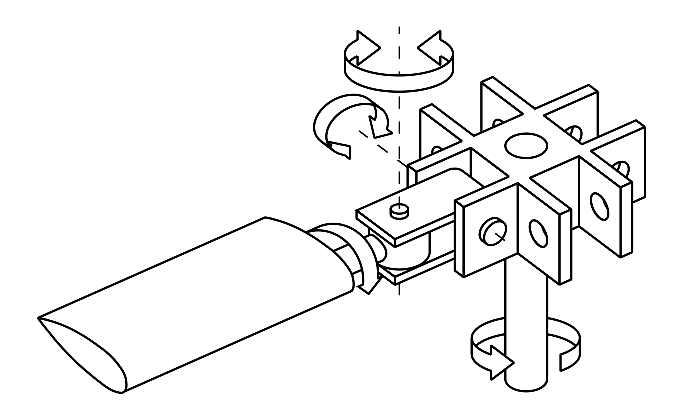
\includegraphics[width=110mm]{eps/rotor_hub_hinges.eps}
  \caption{Rotor blade hinges}
\end{figure}

Neglecting blade flapping motions occuring more frequent than once per revolution flapping angle can be expressed as:

\begin{equation}
\beta \left( \Psi \right)
=
\beta_0 + \beta_{1c} \cos \Psi + \beta_{1s} \sin \Psi 
\end{equation}

\begin{figure}[h!]
  \centering
  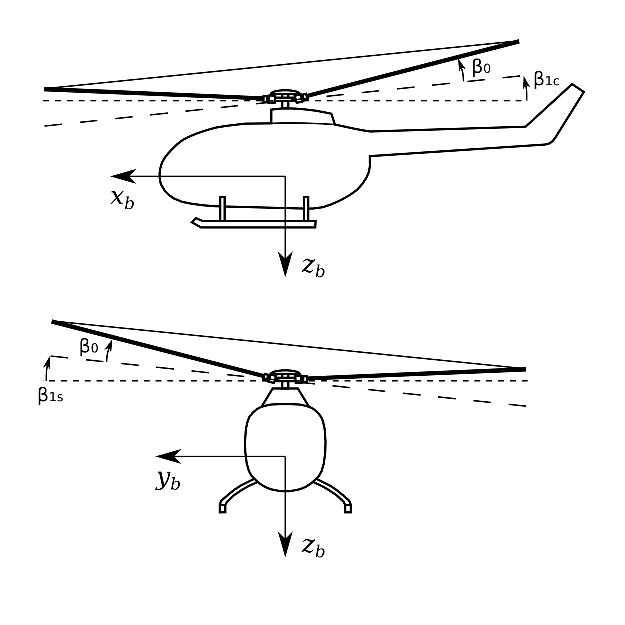
\includegraphics[width=100mm]{eps/rotor_flapping_angles.eps}
  \caption{Rotor disc three degrees of freedom}
\end{figure}
